\documentclass[ignorenonframetext,]{beamer}
\setbeamertemplate{caption}[numbered]
\setbeamertemplate{caption label separator}{: }
\setbeamercolor{caption name}{fg=normal text.fg}
\beamertemplatenavigationsymbolsempty
\usepackage{lmodern}
\usepackage{amssymb,amsmath}
\usepackage{ifxetex,ifluatex}
\usepackage{fixltx2e} % provides \textsubscript
\ifnum 0\ifxetex 1\fi\ifluatex 1\fi=0 % if pdftex
  \usepackage[T1]{fontenc}
  \usepackage[utf8]{inputenc}
\else % if luatex or xelatex
  \ifxetex
    \usepackage{mathspec}
  \else
    \usepackage{fontspec}
  \fi
  \defaultfontfeatures{Ligatures=TeX,Scale=MatchLowercase}
\fi
% use upquote if available, for straight quotes in verbatim environments
\IfFileExists{upquote.sty}{\usepackage{upquote}}{}
% use microtype if available
\IfFileExists{microtype.sty}{%
\usepackage{microtype}
\UseMicrotypeSet[protrusion]{basicmath} % disable protrusion for tt fonts
}{}
\newif\ifbibliography
\hypersetup{
            pdftitle={Longitudinal Data: Repeated Measures},
            pdfauthor={Alan Hubbard},
            pdfborder={0 0 0},
            breaklinks=true}
\urlstyle{same}  % don't use monospace font for urls
\usepackage{color}
\usepackage{fancyvrb}
\newcommand{\VerbBar}{|}
\newcommand{\VERB}{\Verb[commandchars=\\\{\}]}
\DefineVerbatimEnvironment{Highlighting}{Verbatim}{commandchars=\\\{\}}
% Add ',fontsize=\small' for more characters per line
\usepackage{framed}
\definecolor{shadecolor}{RGB}{248,248,248}
\newenvironment{Shaded}{\begin{snugshade}}{\end{snugshade}}
\newcommand{\KeywordTok}[1]{\textcolor[rgb]{0.13,0.29,0.53}{\textbf{#1}}}
\newcommand{\DataTypeTok}[1]{\textcolor[rgb]{0.13,0.29,0.53}{#1}}
\newcommand{\DecValTok}[1]{\textcolor[rgb]{0.00,0.00,0.81}{#1}}
\newcommand{\BaseNTok}[1]{\textcolor[rgb]{0.00,0.00,0.81}{#1}}
\newcommand{\FloatTok}[1]{\textcolor[rgb]{0.00,0.00,0.81}{#1}}
\newcommand{\ConstantTok}[1]{\textcolor[rgb]{0.00,0.00,0.00}{#1}}
\newcommand{\CharTok}[1]{\textcolor[rgb]{0.31,0.60,0.02}{#1}}
\newcommand{\SpecialCharTok}[1]{\textcolor[rgb]{0.00,0.00,0.00}{#1}}
\newcommand{\StringTok}[1]{\textcolor[rgb]{0.31,0.60,0.02}{#1}}
\newcommand{\VerbatimStringTok}[1]{\textcolor[rgb]{0.31,0.60,0.02}{#1}}
\newcommand{\SpecialStringTok}[1]{\textcolor[rgb]{0.31,0.60,0.02}{#1}}
\newcommand{\ImportTok}[1]{#1}
\newcommand{\CommentTok}[1]{\textcolor[rgb]{0.56,0.35,0.01}{\textit{#1}}}
\newcommand{\DocumentationTok}[1]{\textcolor[rgb]{0.56,0.35,0.01}{\textbf{\textit{#1}}}}
\newcommand{\AnnotationTok}[1]{\textcolor[rgb]{0.56,0.35,0.01}{\textbf{\textit{#1}}}}
\newcommand{\CommentVarTok}[1]{\textcolor[rgb]{0.56,0.35,0.01}{\textbf{\textit{#1}}}}
\newcommand{\OtherTok}[1]{\textcolor[rgb]{0.56,0.35,0.01}{#1}}
\newcommand{\FunctionTok}[1]{\textcolor[rgb]{0.00,0.00,0.00}{#1}}
\newcommand{\VariableTok}[1]{\textcolor[rgb]{0.00,0.00,0.00}{#1}}
\newcommand{\ControlFlowTok}[1]{\textcolor[rgb]{0.13,0.29,0.53}{\textbf{#1}}}
\newcommand{\OperatorTok}[1]{\textcolor[rgb]{0.81,0.36,0.00}{\textbf{#1}}}
\newcommand{\BuiltInTok}[1]{#1}
\newcommand{\ExtensionTok}[1]{#1}
\newcommand{\PreprocessorTok}[1]{\textcolor[rgb]{0.56,0.35,0.01}{\textit{#1}}}
\newcommand{\AttributeTok}[1]{\textcolor[rgb]{0.77,0.63,0.00}{#1}}
\newcommand{\RegionMarkerTok}[1]{#1}
\newcommand{\InformationTok}[1]{\textcolor[rgb]{0.56,0.35,0.01}{\textbf{\textit{#1}}}}
\newcommand{\WarningTok}[1]{\textcolor[rgb]{0.56,0.35,0.01}{\textbf{\textit{#1}}}}
\newcommand{\AlertTok}[1]{\textcolor[rgb]{0.94,0.16,0.16}{#1}}
\newcommand{\ErrorTok}[1]{\textcolor[rgb]{0.64,0.00,0.00}{\textbf{#1}}}
\newcommand{\NormalTok}[1]{#1}
\usepackage{graphicx,grffile}
\makeatletter
\def\maxwidth{\ifdim\Gin@nat@width>\linewidth\linewidth\else\Gin@nat@width\fi}
\def\maxheight{\ifdim\Gin@nat@height>\textheight0.8\textheight\else\Gin@nat@height\fi}
\makeatother
% Scale images if necessary, so that they will not overflow the page
% margins by default, and it is still possible to overwrite the defaults
% using explicit options in \includegraphics[width, height, ...]{}
\setkeys{Gin}{width=\maxwidth,height=\maxheight,keepaspectratio}

% Prevent slide breaks in the middle of a paragraph:
\widowpenalties 1 10000
\raggedbottom

\AtBeginPart{
  \let\insertpartnumber\relax
  \let\partname\relax
  \frame{\partpage}
}
\AtBeginSection{
  \ifbibliography
  \else
    \let\insertsectionnumber\relax
    \let\sectionname\relax
    \frame{\sectionpage}
  \fi
}
\AtBeginSubsection{
  \let\insertsubsectionnumber\relax
  \let\subsectionname\relax
  \frame{\subsectionpage}
}

\setlength{\parindent}{0pt}
\setlength{\parskip}{6pt plus 2pt minus 1pt}
\setlength{\emergencystretch}{3em}  % prevent overfull lines
\providecommand{\tightlist}{%
  \setlength{\itemsep}{0pt}\setlength{\parskip}{0pt}}
\setcounter{secnumdepth}{0}
\usepackage{pdfpages}

\title{Longitudinal Data: Repeated Measures}
\subtitle{Linear Models with repeated measures}
\author{Alan Hubbard}
\date{Oct 2, 2018}

\begin{document}
\frame{\titlepage}

\begin{frame}[fragile]

\begin{Shaded}
\begin{Highlighting}[]
\NormalTok{dat <-}\StringTok{ }\KeywordTok{read_csv}\NormalTok{(}\StringTok{"dental.csv"}\NormalTok{)}
\KeywordTok{tbl_df}\NormalTok{(dat)}
\end{Highlighting}
\end{Shaded}

\begin{verbatim}
## # A tibble: 108 x 5
##    obsno child   age distance gender
##    <int> <int> <int>    <dbl>  <int>
##  1     1     1     8     21        0
##  2     2     1    10     20        0
##  3     3     1    12     21.5      0
##  4     4     1    14     23        0
##  5     5     2     8     21        0
##  6     6     2    10     21.5      0
##  7     7     2    12     24        0
##  8     8     2    14     25.5      0
##  9     9     3     8     20.5      0
## 10    10     3    10     24        0
## # ... with 98 more rows
\end{verbatim}

\end{frame}

\begin{frame}{Data Notation}

\begin{itemize}
\tightlist
\item
  child = i (id)
\item
  \(age = X_{ij1}\)
\item
  \(gender = X_{ij2}\): 1 is male, 0 female
\item
  measure of teeth \(distance = Y_{ij}\)
\end{itemize}

\end{frame}

\begin{frame}{Plot the data}

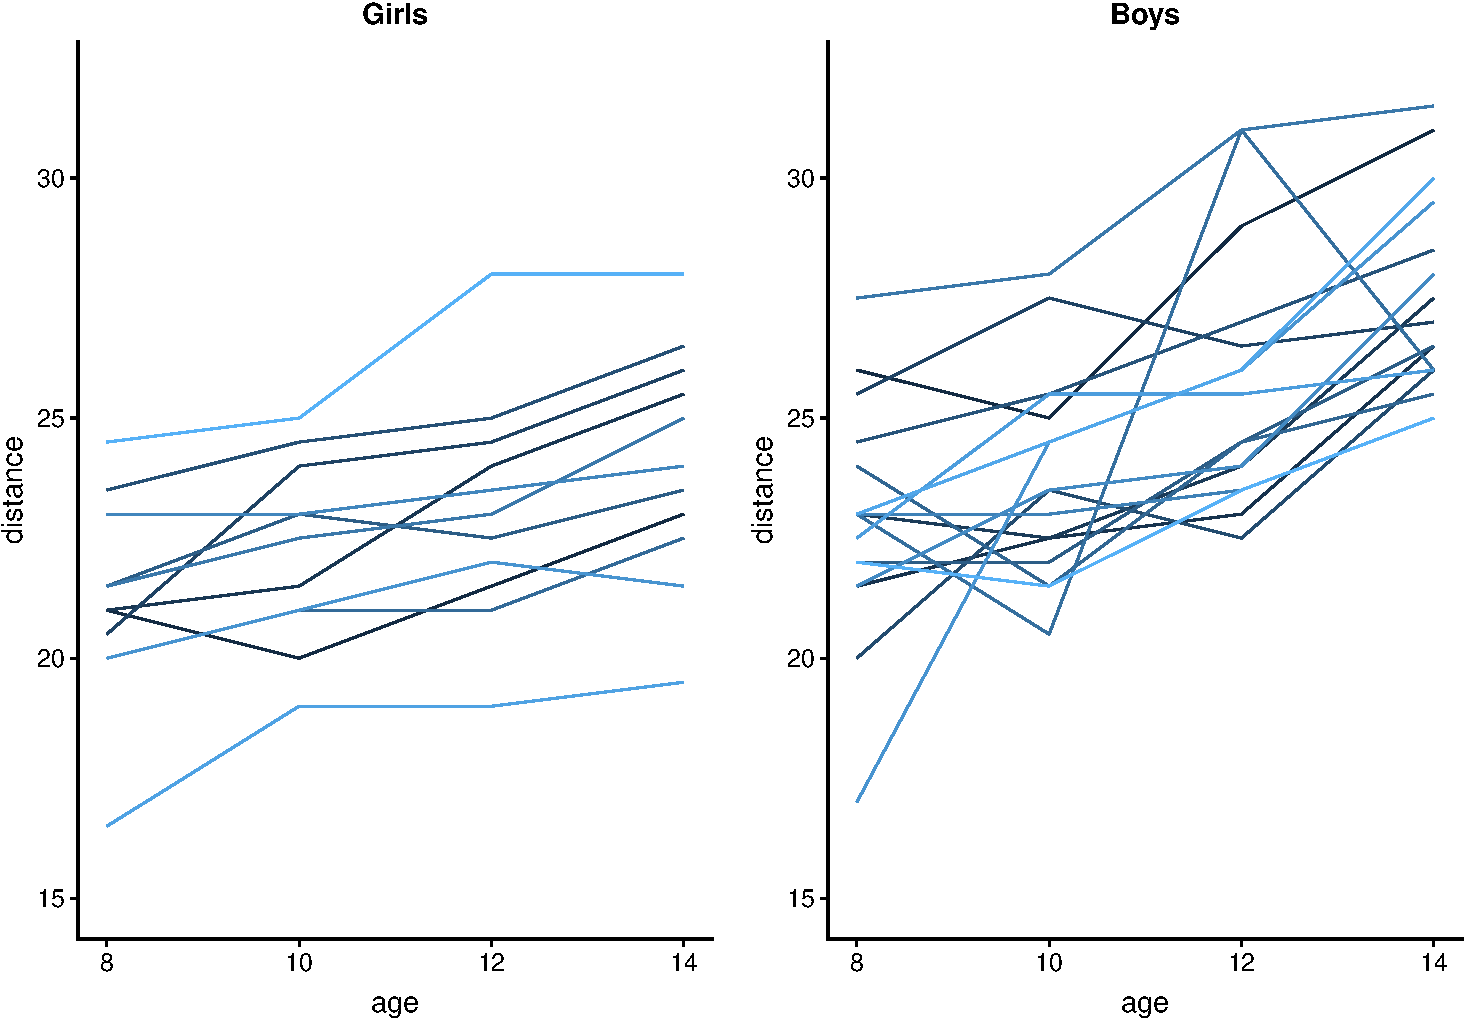
\includegraphics{Chapter5JustCodePart1_files/figure-beamer/plot1-1.pdf}

\end{frame}

\begin{frame}[fragile]{Look at basic summaries with dplyr}

\begin{Shaded}
\begin{Highlighting}[]
\CommentTok{# get number of obs per person and mean}
\NormalTok{sum_dat=}\KeywordTok{group_by}\NormalTok{(dat,child) }\OperatorTok\StringTok{ }\KeywordTok{summarise}\NormalTok{(}\DataTypeTok{mean=}\KeywordTok{mean}\NormalTok{(distance),}\DataTypeTok{n=}\KeywordTok{n}\NormalTok{(),}\DataTypeTok{gender=}\KeywordTok{first}\NormalTok{(gender))}
\KeywordTok{table}\NormalTok{(sum_dat}\OperatorTok{$}\NormalTok{gender)}
\end{Highlighting}
\end{Shaded}

\begin{verbatim}
## 
##  0  1 
## 11 16
\end{verbatim}

\end{frame}

\begin{frame}{Estimate linear model for dental data}

\begin{itemize}
\tightlist
\item
  Again, the model we wanted to estimate is:
\end{itemize}

\[ E(Y_{ij} \mid \vec{X}_{ij}) = \beta_0 +\beta_1 X_{ij1}+\beta_2 X_{ij2} + \beta_3 X_{ij1}X_{ij2} \]

\end{frame}

\begin{frame}[fragile]{Use simple OLS}

\tiny

\begin{Shaded}
\begin{Highlighting}[]
\CommentTok{# First, make interaction term}
\KeywordTok{library}\NormalTok{(RCurl)}
\NormalTok{dat =}\StringTok{ }\NormalTok{dat }\OperatorTok\StringTok{ }\KeywordTok{mutate}\NormalTok{(}\DataTypeTok{inter=}\NormalTok{gender}\OperatorTok{*}\NormalTok{age)}
\NormalTok{ols_fit =}\StringTok{ }\KeywordTok{lm}\NormalTok{(distance }\OperatorTok{~}\StringTok{ }\NormalTok{gender}\OperatorTok{+}\NormalTok{age}\OperatorTok{+}\NormalTok{inter, }\DataTypeTok{data=}\NormalTok{dat)}
\KeywordTok{summary}\NormalTok{(ols_fit)}
\end{Highlighting}
\end{Shaded}

\begin{verbatim}
## 
## Call:
## lm(formula = distance ~ gender + age + inter, data = dat)
## 
## Residuals:
##     Min      1Q  Median      3Q     Max 
## -5.6156 -1.3219 -0.1682  1.3299  5.2469 
## 
## Coefficients:
##             Estimate Std. Error t value Pr(>|t|)    
## (Intercept)  17.3727     1.7080  10.171  < 2e-16 ***
## gender       -1.0321     2.2188  -0.465  0.64279    
## age           0.4795     0.1522   3.152  0.00212 ** 
## inter         0.3048     0.1977   1.542  0.12608    
## ---
## Signif. codes:  0 '***' 0.001 '**' 0.01 '*' 0.05 '.' 0.1 ' ' 1
## 
## Residual standard error: 2.257 on 104 degrees of freedom
## Multiple R-squared:  0.4227, Adjusted R-squared:  0.4061 
## F-statistic: 25.39 on 3 and 104 DF,  p-value: 2.108e-12
\end{verbatim}

\end{frame}

\begin{frame}[fragile]{Getting estimates of linear combination of
coefficients}

\tiny

\begin{Shaded}
\begin{Highlighting}[]
\NormalTok{## Note how the algebra is entered into function}
\NormalTok{### For boys}
\NormalTok{lin.boys=}\KeywordTok{glht}\NormalTok{(ols_fit, }\DataTypeTok{linfct =} \KeywordTok{c}\NormalTok{(}\StringTok{"6*age +6*inter=0"}\NormalTok{))}
\CommentTok{#summary(lin.boys)}
\KeywordTok{confint}\NormalTok{(lin.boys)  }
\end{Highlighting}
\end{Shaded}

\begin{verbatim}
## 
##   Simultaneous Confidence Intervals
## 
## Fit: lm(formula = distance ~ gender + age + inter, data = dat)
## 
## Quantile = 1.983
## 95% family-wise confidence level
##  
## 
## Linear Hypotheses:
##                          Estimate lwr    upr   
## 6 * age + 6 * inter == 0 4.7063   3.2051 6.2074
\end{verbatim}

\end{frame}

\begin{frame}[fragile]{Repeat for girls}

In this case,
\[ E(Y_{ij} \mid X_{ij1}=age+6,X_{ij2}=0) -  E(Y_{ij} \mid X_{ij1}=age,X_{ij2}=0) \]
\[ =  6*\beta_1\]

\tiny

\begin{Shaded}
\begin{Highlighting}[]
\NormalTok{lin.girls=}\KeywordTok{glht}\NormalTok{(ols_fit, }\DataTypeTok{linfct =} \KeywordTok{c}\NormalTok{(}\StringTok{"6*age=0"}\NormalTok{))}
\CommentTok{#summary(lin.girls)}
\KeywordTok{confint}\NormalTok{(lin.girls)  }
\end{Highlighting}
\end{Shaded}

\begin{verbatim}
## 
##   Simultaneous Confidence Intervals
## 
## Fit: lm(formula = distance ~ gender + age + inter, data = dat)
## 
## Quantile = 1.983
## 95% family-wise confidence level
##  
## 
## Linear Hypotheses:
##              Estimate lwr    upr   
## 6 * age == 0 2.8773   1.0668 4.6877
\end{verbatim}

The results suggest that the mean change in the distance for boys is
4.76 (95\% 3.20-6.21) and that for girls is 2.88 (95\% 1.07-4.69).

\end{frame}

\begin{frame}[fragile]{Inference sandwich estimator}

\tiny

\begin{Shaded}
\begin{Highlighting}[]
\CommentTok{# Read in user written function using lmtest and }
\CommentTok{# sandwich packages that return both information }
\CommentTok{# on coefficients and estimates of linear}
\CommentTok{# combination of coefficients using}
\CommentTok{# clustered/robust variance estimates}
\KeywordTok{source}\NormalTok{(}\StringTok{"clx.R"}\NormalTok{)}
\KeywordTok{source}\NormalTok{(}\StringTok{"clx_lincom.R"}\NormalTok{)}

\KeywordTok{clx}\NormalTok{(ols_fit, }\DecValTok{1}\NormalTok{, dat}\OperatorTok{$}\NormalTok{child)}
\end{Highlighting}
\end{Shaded}

\begin{verbatim}
## 
## t test of coefficients:
## 
##              Estimate Std. Error t value  Pr(>|t|)    
## (Intercept) 17.372727   0.749604 23.1759 < 2.2e-16 ***
## gender      -1.032102   1.424137 -0.7247   0.47025    
## age          0.479545   0.065257  7.3486 4.712e-11 ***
## inter        0.304830   0.120799  2.5234   0.01313 *  
## ---
## Signif. codes:  0 '***' 0.001 '**' 0.01 '*' 0.05 '.' 0.1 ' ' 1
\end{verbatim}

\begin{Shaded}
\begin{Highlighting}[]
\CommentTok{# Robust estimate for change in mean}
\CommentTok{# for 6 year increase in age for}
\CommentTok{# boys}
\KeywordTok{clx.lincom}\NormalTok{(ols_fit, }\DecValTok{1}\NormalTok{,dat}\OperatorTok{$}\NormalTok{child, }\KeywordTok{c}\NormalTok{(}\DecValTok{0}\NormalTok{,}\DecValTok{0}\NormalTok{,}\DecValTok{6}\NormalTok{,}\DecValTok{6}\NormalTok{))}
\end{Highlighting}
\end{Shaded}

\begin{verbatim}
##      Est      CI                pvalue  
## [1,] "4.7063" "3.5108 - 5.9017" "0.0000"
\end{verbatim}

\end{frame}

\begin{frame}{Comparison of results}

\begin{itemize}
\tightlist
\item
  If one looks at the age coefficient, one can see that the robust SE is
  much smaller than the naive one returned by standard OLS: 0.065 vs
  0.152.\\
\item
  We can also compare the results of the estimate of\\
  \[ =  6*\beta_1 + 6*\beta_3\] and we see the CI based upon the robust
  estimates that account for dependence is 3.511-5.911 versus
  3.205-6.207, so for this parameter, the CI gets bigger when the SE is
  estimated correctly.
\end{itemize}

\end{frame}

\end{document}
